\section{Knowledge Circuits Elucidate Internal Mechanisms for Knowledge Editing}
\label{sec:edit_experiment}
% Having identified the circuit responsible for representing a specific piece of knowledge, we 
In this section, our objective is to evaluate the impact of previous knowledge editing methods and validate the effectiveness of knowledge circuits.
We aim to understand why these methods may fail in certain cases and settings, which can also help deepen the understanding of the knowledge circuit.
%Through this process, we also aim to deepen our understanding of the knowledge circuit.
\begin{figure}
    \centering
    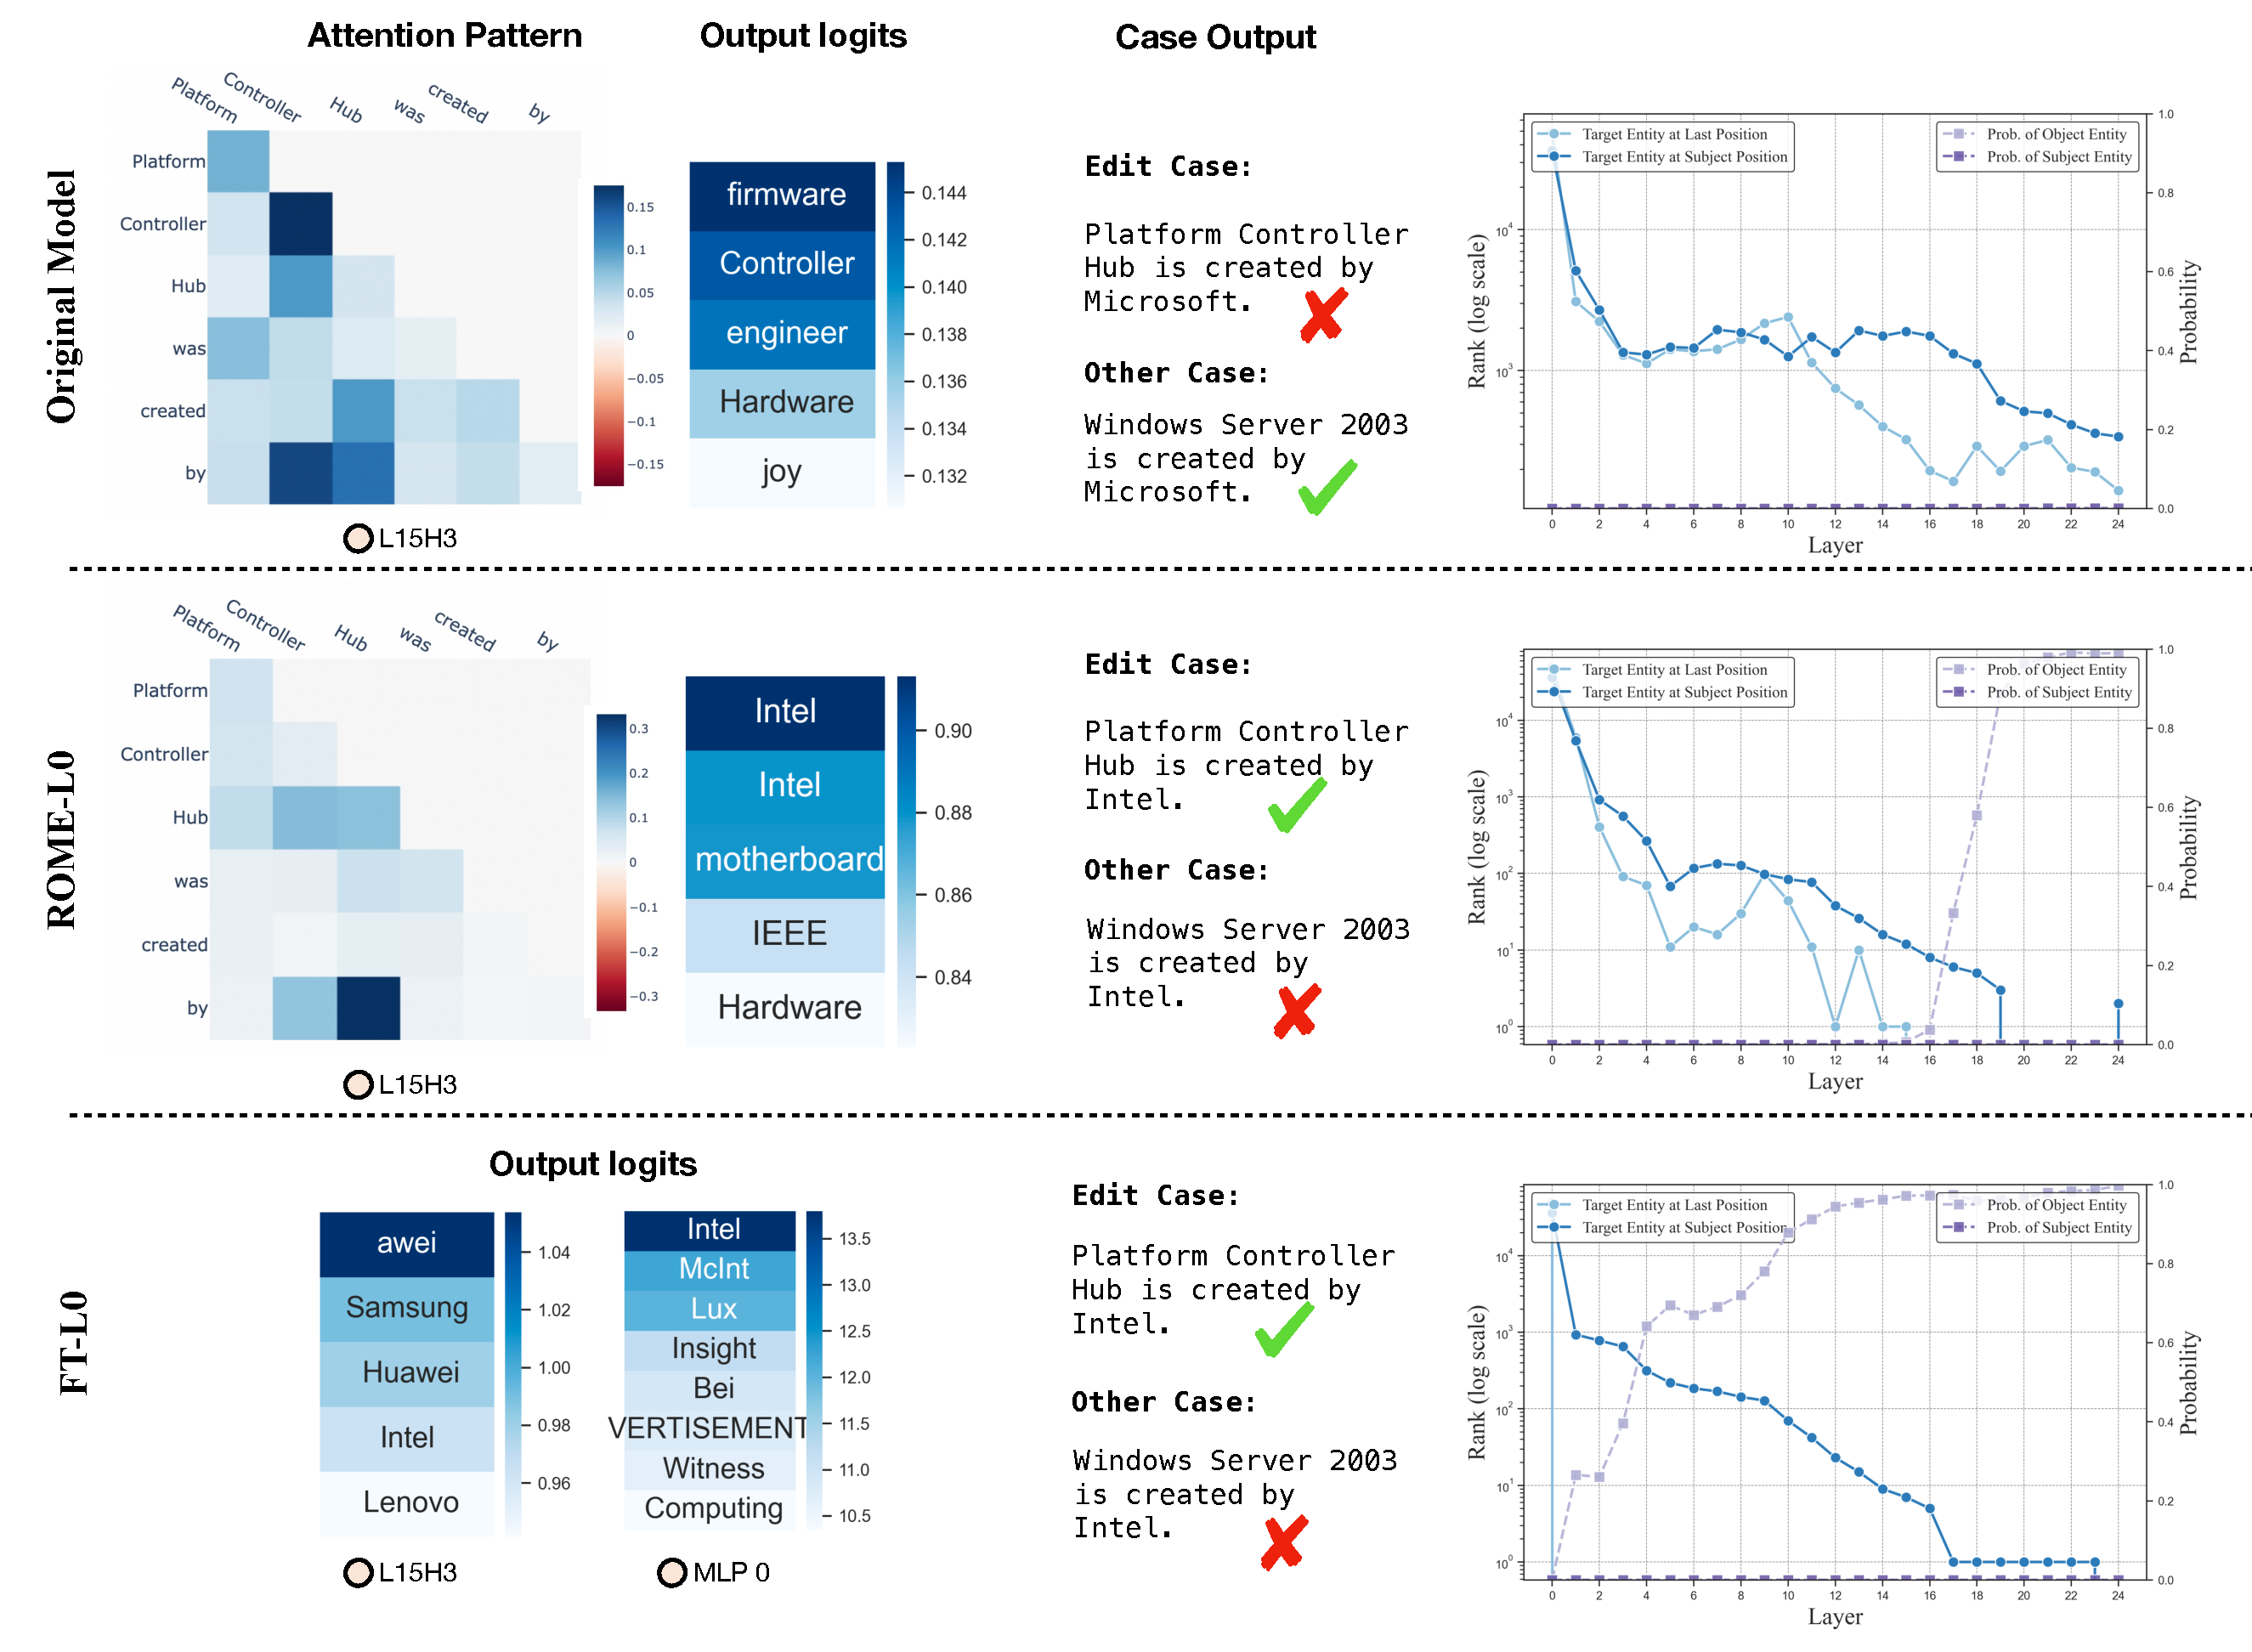
\includegraphics[width=0.95\linewidth]{Figure/parameter-edit.pdf}
    \caption{Different behaviors when we edit the language model.
    In the original model, we can see the mover head L15H3 actually move the original token \nl{Controller} and other information, while for ROME, we observe the mover head select the correct information \nl{Intel}, which means ROME \textbf{successfully added the \nl{Intel} to model}. 
    For the FT layer-0 editing, we can find this method \textbf{directly write the edited knowledge into edited component}.
    However, we find these two editing methods would affect other unrelated input \nl{Windows server is created by?} }
    \label{fig:parameter-edit}
\end{figure}
\paragraph{Single Factual Knowledge Editing.}
\label{parameter edit}
Here, we adopt the ROME method~\cite{meng2022locating} and FT-M~\cite{knowledge_editing_survey_2}, which aim to edit the MLP layers in the language model.
The most important hyper-parameter in knowledge editing is the layer, as the same method's performance varies significantly via the layers.
Here, we evaluate the performance of different editing layers and their effectiveness.
We compare the knowledge circuits computed by the edited model with the original one, and we present results in Figure~\ref{fig:parameter-edit} and report details in Appendix~\ref{app:edit_experiments}.
As discussed in the previous part, the early-to-middle layers are the main part of aggregating the target entity $o$ to the top rank.
In the original model, the probability of the target entity \nl{Intel} is nearly zero, and the model fails to elevate it to the top rank in the vocabulary.
Editing the model with ROME and FT-M both give us the correct answer but we can view different scenarios for their knowledge circuits.
For \textbf{ROME}, as the correct information is added to the subject position, we can recognize a \textbf{behavior of the Mover Head shifts from copying to extracting the edited information from the subject position}.
This information gradually aggregates through the subsequent layers, and by layer 15, \nl{Intel} emerges as the top-ranked entity with its probability increasing significantly.
Specially, before editing, the mover head L15H3 attends to the \nl{controller} token and returns \nl{controller} as the output, while in the edited model, the attention head's output moves to the \nl{Intel}, which means the model gains the information at the subject space.
For FT-M, the edited model tends to directly write the knowledge into the specific component, which would greatly dominate the following component in the model.
As shown in Figure~\ref{fig:parameter-edit}, the output logits in MLP-0 for \nl{Intel} are more than 10, and it emerges as the top rank in the residual stream directly. 
This phenomenon can be found in different knowledge types and layers and we report results in Appendix \ref{appendix:Edit Cases}.
However, the added knowledge may have the risk of influencing unrelated knowledge.
When we test another fact \nl{Windows server}, the model still tends to give us the \nl{Intel} answer, demonstrating the overfitting problem.
This finding supports previous analysis regarding the correlation between localization and editing~\cite{hase2023does}, suggesting that edits may not alter the storage but merely add signals into the knowledge circuits.

\paragraph{Multi-hop Factual Knowledge Editing.}
Multi-hop knowledge editing poses a challenging scenario~\cite{yao-etal-2023-editing,10.1162/tacl_a_00644,zhong-etal-2023-mquake}, wherein we edit the model with new knowledge, yet the model struggles to perform reasoning using the edited information.
We analyze multi-hop questions in language models \cite{yang2024large,ju2024investigating} to understand why current editing methods fail in these scenarios.
For instance, given the fact (Thierry Mugle, \nl{home country}, France), we edit the fact to another country, such as (Thierry Mugle, \nl{home country}, France $\rightarrow$ China).
We then assess the model's performance on questions based on the edited knowledge, including \nl{The official currency of the home country of Thierry Mugle is} and \nl{The capital city of the home country of Thierry Mugle is}.
While the unedited model could correctly answer these questions, we observe that the edited model would provide the answer \nl{China} for subsequent hop reasoning.
We find that the mover head in the original multi-hop reasoning circuit initially extracts the second-hop answer but, after editing, extracts \nl{China}, demonstrating that the edited information dominantly saturates and influences the circuit.
Furthermore, we observe an intriguing phenomenon: \textbf{even in the original model's multi-hop reasoning settings, it would directly provide the answer if we remove the context of the first-hop texts} (Details in Appendix~\ref{app:multi-hop}).
This further confirms the findings that the model relies on relational and subject-related information, regardless of grammatical adherence.
% \begin{wrapfigure}{r}{0.4\columnwidth}
%     \centering
%     \vspace{-0.3cm}
%     \includesvg[width=0.99\linewidth]{Figure/halluciantion.svg}
%     \caption{A competition for the error and correct information. We can find at the specific layer, the error information would surpass the correct one. }
%     \label{fig:halluciantion}
%     \vspace{-0.5cm}
% \end{wrapfigure}